\documentclass[11pt]{article}
\usepackage{graphicx}

\begin{document}
	
	\begin{center}
		\begin{Large}
			Assignment No 5
		\end{Large}
	\end{center}•
	Aim: Generating abstract syntax tree using LEX and YACC\\
	
	\noindent
	Objective:
	\begin{enumerate}
		\item To understand the concept of syntax tree..
		\item To generate an abstract syntax tree for the given arithmetic expression.
	\end{enumerate}•
	
	\noindent
	Software Requirement:
	\begin{enumerate}
		\item Linux Operating System
		\item Lex compiler
		\item Yacc compiler
	\end{enumerate}•
	
	\noindent
	Mathematical Model:\\
	Consider a set S consisting of all the elements related to a program.The mathematical model is given as below,\\ S={s,e,X,Y,Fme,DD,NDD,Mem shared}\\ Where, s = Initial State\\ e = End State\\
	X	= Input data. Here it is any valid arithmetic expression.\\
	Y	= Output.Here output is pre-order or post-order traversal of syntax tree.\\
	Fme = Algorithm/Function used in program.for eg.{create(), preorder(), postorder()}\\
	DD = Deterministic Data\\
	NDD = Non deterministic Data Mem shared = Memory shared by processor.\\
	
	
	\noindent
	Theory:\\
	Abstract Syntax Tree :\\
	An (absract) syntax tree is a condensed form of parse tree useful for representing language constructs.In syntax tree, operators and keywords do not appear as leaves, but rather are associated with the interior node that would be the parent of those leaves in the parse tree.\\
	
	\noindent
	For Example :\\
	a syntax-tree node representing an expression E1 + E2 has label + and two children representing the sub expressions E1 and E2.\\
	Abstract syntax trees are data structures widely used in compilers, due to their property of representing the structure of program code.An AST is usually the result of syntax analysis phase of a compiler.It ofen serves as an intermediate representation of the program trough several stages that the compiler requires, and has a strong impact on the final output of the compiler.\\
	
	\noindent
	Constructing Syntax Trees for Expressions :\\
	
	The construction of syntax tree for an expression is similar to the translation of the expression into postfix form.
	Each node in a syntax tree can be implemented as a record with the several fields.In the node for an operator, one can identifies the operator and the remaining fields contain pointers to the nodes for the operands. The operator is often called as the label of the node.When used for translation, the nodes in a syntax may have additional fields to hold the values of attributes attached to the node.\\
	
	\noindent
	Syntax Directed Definitions for generating abstract syntax tree :\\
	
	Following table contains an S-attributed defination constructs syntax trees for a simple expression grammar involving only the binary operators + and -. As usual, these operators are at the same precedence level and are jointly left associative. All nonterminals have one synthesized attribute node, which represents a node of the syntax tree.\\
	
	\begin{center}
		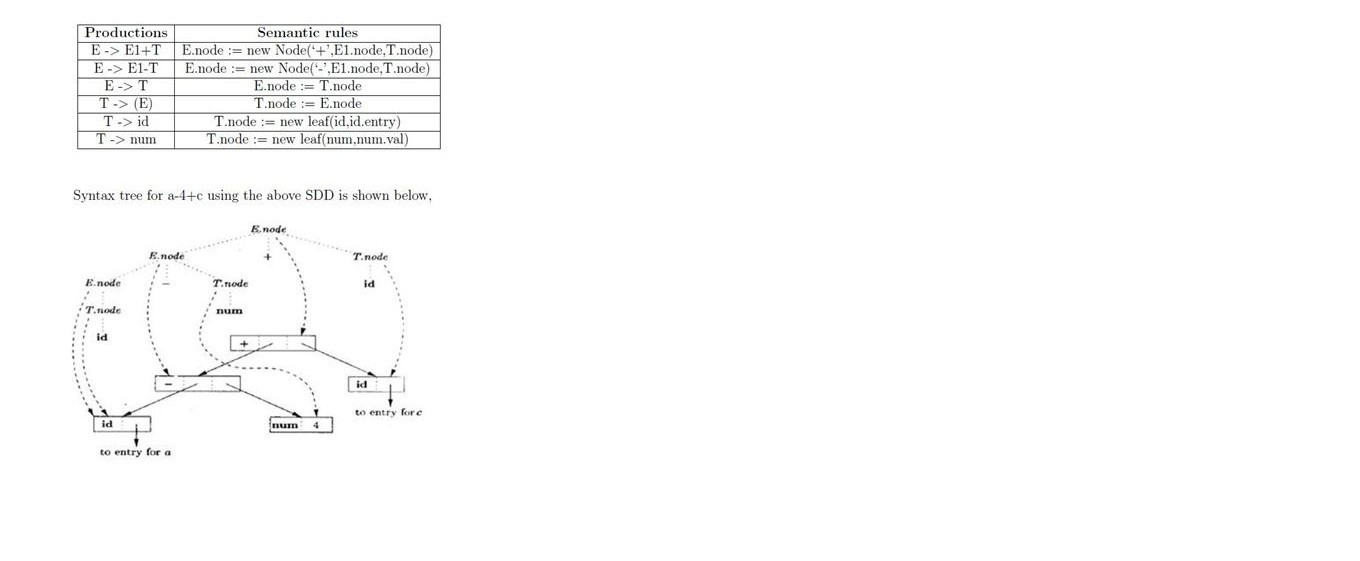
\includegraphics{tem.png}
	\end{center}•
	
	\noindent
	Steps in the construction of the syntax tree for a-4+c :\\
	
	If the rules are evaluated during a post order traversal of the parse tree, or with reductions during a bottom-up parse, then the sequence of steps shown below ends with p5 pointing to the root of the constructed syntax tree.\\
	\begin{enumerate}
		\item p1 = new Leaf(id,entry-a);
		\item p2 = new Leaf(num,4);
		\item p3 = new Node(‘-’,p1,p2);
		\item p4 = new Leaf (id,entry-c);
		\item p5 = new Node(‘+’,p3,p4);
		
	\end{enumerate}•
	
	\noindent
	Command :\\
	\$ lex $<program name>.$l\\
	\$ yacc -d $<program name>$.y\\
	\$ gcc lex.yy.c y.tab.c -ll -ly\\
	\$ ./a.out\\
	
	\noindent
	CONCLUSION :\\
	Thus, we have generated an abstract syntax tree for the given arithnetic expression using LEX and YACC.\\
	
	\begin{center}
		\begin{tabular}{|c|c|c|c|c|}
			•$Roll$ $No$ & $Name$ $of$ $Student$ & $Date$ $of$ $performance$ & $Date$ $of$ $Checking$ & $Signature$ $of$ $Staff$ \\ \hline
			$BECOC357$ & Sunny Shah& 22 / 09 / 2017 & 22 / 09 / 2017&     \\ \hline
		\end{tabular}•
	\end{center}•
	\newpage
	\section{PLAGARISM REPORT :}
	\begin{figure}[h!]
		\centering
		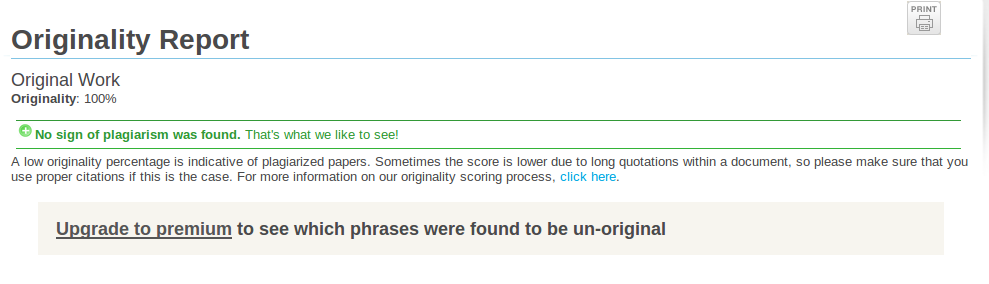
\includegraphics[height=5in,width=6in]{plagiarism5.png}
		\caption{Plagarism Checker www.smallseotools.com/plagarism-checker}
	\end{figure}
	\newpage
\end{document}
